\documentclass{article}
\usepackage[utf8x]{inputenc}
\usepackage{ucs}
\usepackage{amsmath} 
\usepackage{amsfonts}
\usepackage{marvosym}
\usepackage{wasysym}
\usepackage{upgreek}
\usepackage[english,russian]{babel}
\usepackage{graphicx}
\usepackage{float}
\usepackage{textcomp}
\usepackage{hyperref}
\usepackage{geometry}
  \geometry{left=2cm}
  \geometry{right=1.5cm}
  \geometry{top=1cm}
  \geometry{bottom=2cm}
\usepackage{tikz}
\usepackage{ccaption}
\usepackage{multicol}

\hypersetup{
   colorlinks=true,
   citecolor=blue,
   linkcolor=black,
   urlcolor=blue
}

\usepackage{listings}
%\setlength{\columnsep}{1.5cm}
%\setlength{\columnseprule}{0.2pt}

\usepackage[absolute]{textpos}

\usepackage{colortbl,graphicx,tikz}
\definecolor{X}{rgb}{.5,.5,.5}


\begin{document}
\pagenumbering{gobble}
\lstset{
  language=C,                % choose the language of the code
  basicstyle=\linespread{1.1}\ttfamily,
  columns=fixed,
  fontadjust=true,
  basewidth=0.5em,
  keywordstyle=\color{blue}\bfseries,
  commentstyle=\color{gray},
  stringstyle=\ttfamily\color{orange!50!black},
  showstringspaces=false,
  numbersep=5pt,
  numberstyle=\tiny\color{black},
  numberfirstline=true,
  stepnumber=1,                   % the step between two line-numbers.        
  numbersep=10pt,                  % how far the line-numbers are from the code
  backgroundcolor=\color{white},  % choose the background color. You must add \usepackage{color}
  showstringspaces=false,         % underline spaces within strings
  captionpos=b,                   % sets the caption-position to bottom
  breaklines=true,                % sets automatic line breaking
  breakatwhitespace=true,         % sets if automatic breaks should only happen at whitespace
  xleftmargin=.2in,
  extendedchars=\true,
  keepspaces = true,
}
\lstset{literate=%
   *{0}{{{\color{red!20!violet}0}}}1
    {1}{{{\color{red!20!violet}1}}}1
    {2}{{{\color{red!20!violet}2}}}1
    {3}{{{\color{red!20!violet}3}}}1
    {4}{{{\color{red!20!violet}4}}}1
    {5}{{{\color{red!20!violet}5}}}1
    {6}{{{\color{red!20!violet}6}}}1
    {7}{{{\color{red!20!violet}7}}}1
    {8}{{{\color{red!20!violet}8}}}1
    {9}{{{\color{red!20!violet}9}}}1
}
\newpage

\title{Семинар \#8: Указатели и динамическое выделение памяти. Домашнее задание.\vspace{-5ex}}\date{}\maketitle
\section*{Память}
Как выглядит память, инициализируемая при создании следующих переменных (в системе с порядком байт Little Endian):
\begin{multicols}{2}
\begin{enumerate}
\item \texttt{int a = 0x11223344;}
\item \texttt{int b = 123456789;}
\item \texttt{int array[3] = \{10, 2000, 65535}\};
\item \texttt{char str[8] = ''Hello``};
\item \texttt{float x = -15.91};
\item \texttt{double y = -15.91};
\item
\begin{verbatim}
struct data
{
    char str[5];
    int number;
};
struct data c = {"Cat", 100000};
\end{verbatim}
\end{enumerate}
\end{multicols}
Память представить в виде последовательности 2-значных шестнадцатиричных чисел. Например число \\
\texttt{int a = 757004;} будет храниться в памяти как \texttt{0x54, 0x82, 0x73, 0x00}. \\ \\
\textit{Подсказка:} Чтобы проверить, как будет выглядеть память, можно создать указатель типа \texttt{char*} на эту память и распечатать каждый байт в виде шестнадцатиричного числа:
\begin{lstlisting}
char* p = (char*)&a;
for (int i = 0; i < sizeof(a); ++i)
{
    printf("0x%02hhx ", p[i]);
}
\end{lstlisting}

\section*{Указатели}

\subsection*{Указатель на \texttt{int}}
\begin{lstlisting}
int a = 1234;
int* p = &a;
\end{lstlisting}
\begin{center}
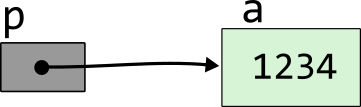
\includegraphics[scale=1]{../../images/pointer_schemes/pointer_to_int.png}
\end{center}

\subsection*{Указатель на указатель на \texttt{int}}
\begin{lstlisting}
int a = 1234;
int* p = &a;
int** q = &p;
\end{lstlisting}
\begin{center}
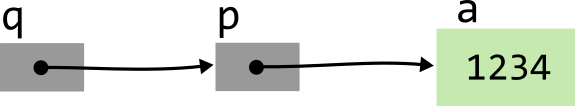
\includegraphics[scale=1]{../../images/pointer_schemes/pointer_to_pointer_to_int.png}
\end{center}

\subsection*{Указатель на элемент массива}
\begin{lstlisting}
int array[5] = ;
int* p = &a[1];
\end{lstlisting}
\begin{center}
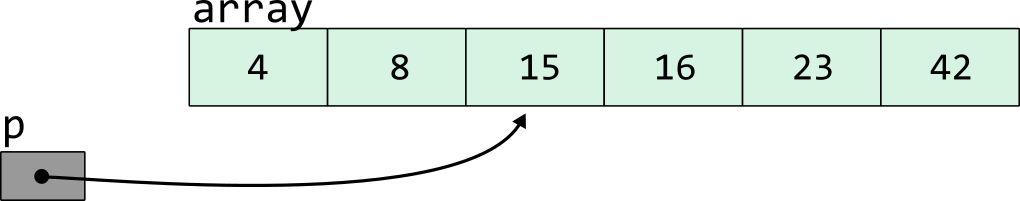
\includegraphics[scale=1]{../../images/pointer_schemes/pointer_to_array_of_ints.png}
\end{center}

\subsection*{Указатель на элемент структуру}
\begin{lstlisting}
struct date
{
	int day, month, year;
};
struct date a = {};
struct date* p = &a;
\end{lstlisting}
\begin{center}
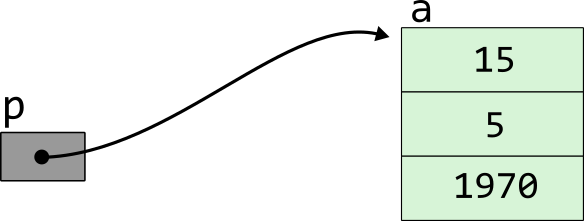
\includegraphics[scale=1]{../../images/pointer_schemes/pointer_to_struct_date.png}
\end{center}

\subsection*{Указатель на элемент структуру \texttt{Movie}}
\begin{lstlisting}
struct movie
{
	char title[50];
	float rating;
	struct date release_date;
};
typedef struct movie Movie;

Movie a = {"Inception", 8.661, {8, 6, 2010}};
Movie* p = &a;
\end{lstlisting}
\begin{center}
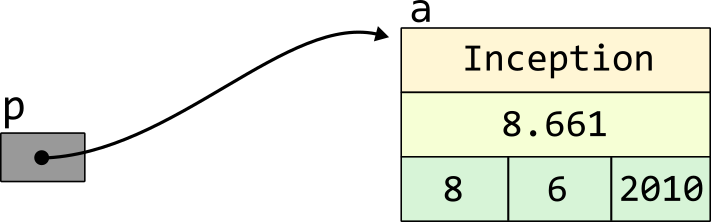
\includegraphics[scale=1]{../../images/pointer_schemes/pointer_to_struct_movie.png}
\end{center}

\subsection*{Указатель на массив структур \texttt{Movie}}
\begin{lstlisting}
struct movie
{
	char title[50];
	float rating;
	struct date release_date;
};
typedef struct movie Movie;

Movie array[3] = {{"Inception", 8.661, {8, 6, 2010}}, 
                  {"Green Mile", 9.062, {6, 12, 1999}}, 
                  {"Leon", 8.679, {14, 9, 1994}};
Movie* p = &array[1];
\end{lstlisting}
\begin{center}
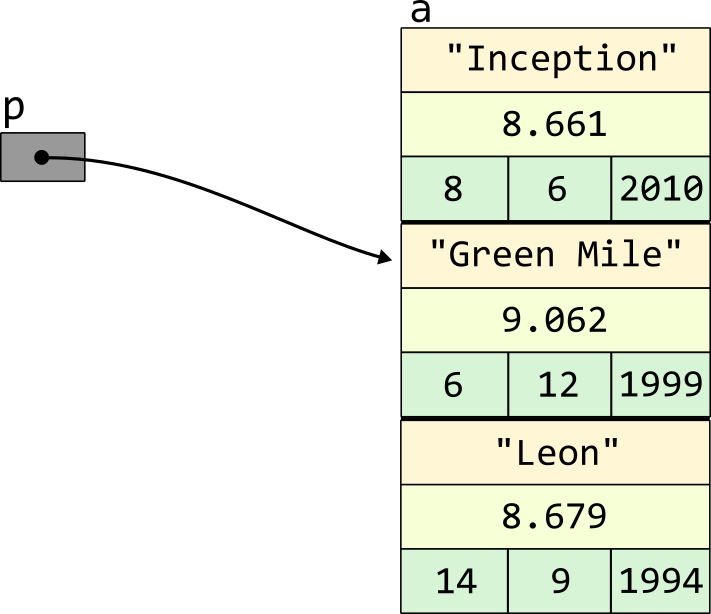
\includegraphics[scale=1]{../../images/pointer_schemes/pointer_to_array_of_struct_movie.png}
\end{center}

\subsection*{Указатель на массив структур, выделенный в куче}
\begin{lstlisting}
struct movie
{
	char title[50];
	float rating;
	struct date release_date;
};
typedef struct movie Movie;

int main()
{
	Movie* p = (Movie*)malloc(3 * sizeof(Movie));
	strcpy(p[0].title, "Inception");
	p[0].rating = 8.661;
	p[0].release_date
Movie array[3] = {{"Inception", 8.661, {8, 6, 2010}}, {"Green Mile", 9.062, {6, 12, 1999}}, 
{"Leon", 8.679, {14, 9, 1994}};
Movie* p = &array[1];
\end{lstlisting}
\begin{center}
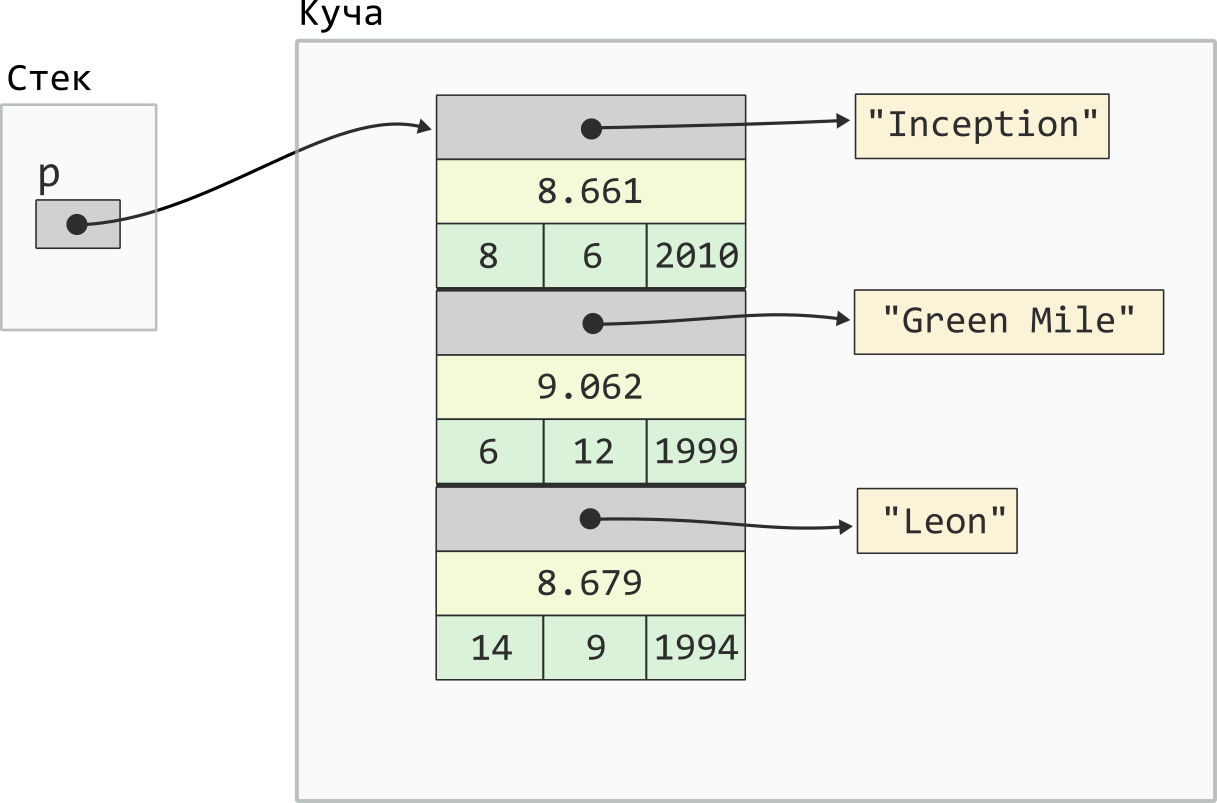
\includegraphics[scale=1]{../../images/pointer_schemes/pointer_to_array_of_struct_movie_charpointers.png}
\end{center}

\begin{center}
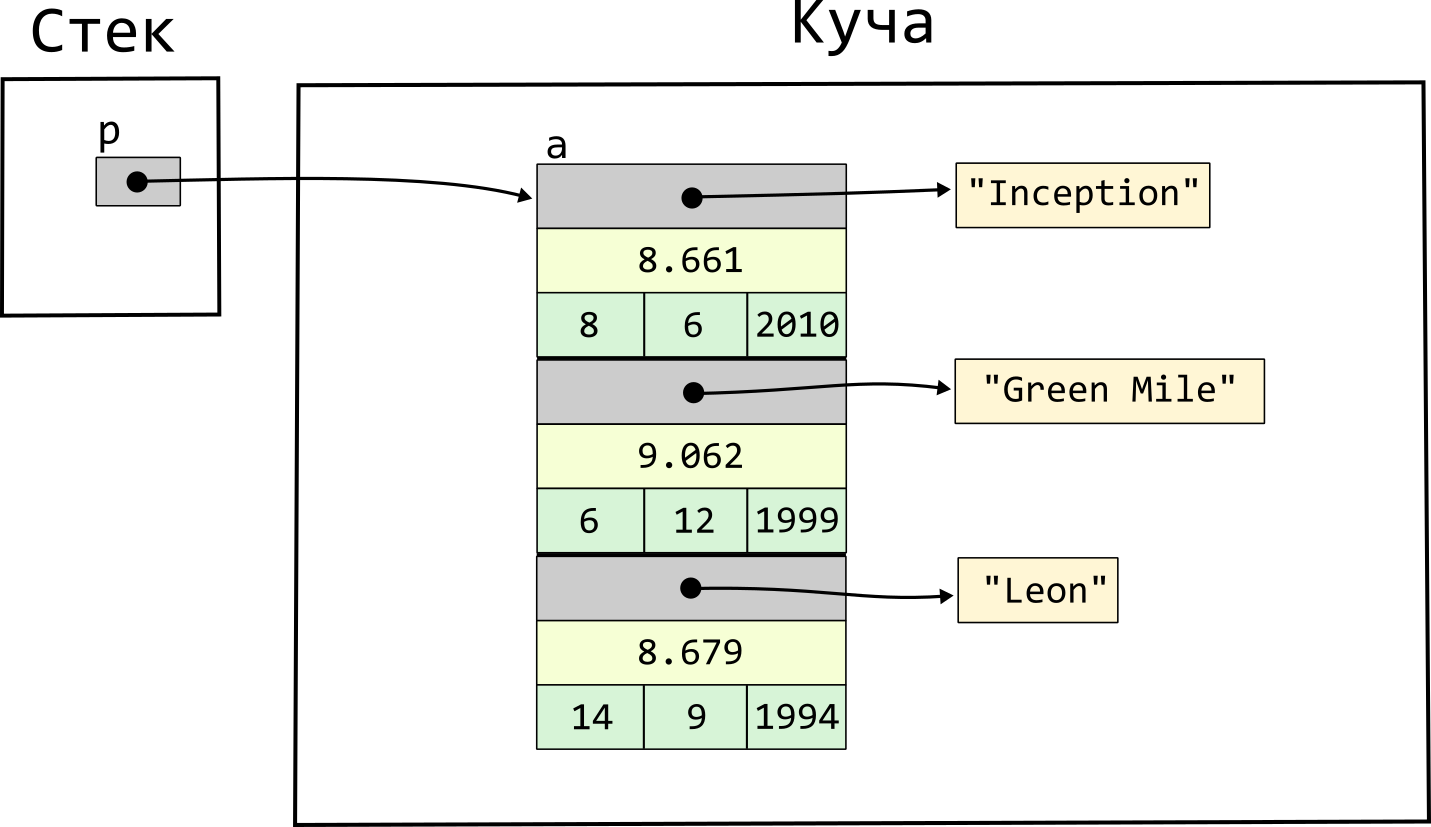
\includegraphics[scale=1]{../../images/pointer_schemes/pointer_to_array_of_struct_movie_charpointers_segments.png}
\end{center}

У каждой переменной есть адрес. Адрес - это номер байта, начиная с которого лежит эта переменная в памяти. Чтобы найти адрес переменной, нужно перед ней поставить знак амперсанда \texttt{\&}. \\
Для хранения адресов в языке C введены специальные переменные, которые называются указатели. Тип переменной указателя = тип той переменной, на которую он `указывает` + звёздочка(\texttt{*}) на конце. Например, указатель, который будет хранить адреса переменных типа \texttt{int} должен иметь тип \texttt{int*}. \\
Чтобы по указателю получить саму переменную, нужно перед указателем поставить звёздочку(\texttt{*}).
\begin{lstlisting}
#include <stdio.h>
int main()
{
    int a = 7;
    printf("Value = %d. Address = %p\n",  a,  &a);
    
    int* pa = &a;
    printf("Value = %d. Address = %p\n", *pa, pa);
}
\end{lstlisting}
Выполните задание из файла \texttt{0pointer\_basics.c}.
\section*{Арифметика указателей}
С указателями можно производить следующие операции:
\begin{itemize}
\item Прибавить или отнять число          \quad             \texttt{p + 2}
\item Вычитать 2 указателя                      \quad       \texttt{p - q}
\item Разыменование (получить то, на что указывает указатель) \quad  \texttt{*p}
\item Квадратные скобки (прибавить число + разыменование): \quad \texttt{p[i] == *(p+i)}
\end{itemize}
Пусть есть одномерный статический массив и указатель на 4-й элемент этого массива:
\begin{lstlisting}
int numbers[6] = {4, 8, 15, 16, 23, 42};
int* p = &numbers[3];
\end{lstlisting}
Чему равны следующие выражения:
\begin{multicols}{3}
\begin{enumerate}
\item \begin{verbatim} numbers[5] \end{verbatim}
\item \begin{verbatim} *p \end{verbatim}
\item \begin{verbatim} *(p+1) \end{verbatim}
\item \begin{verbatim} *(p-2) \end{verbatim}
\item \begin{verbatim} p[0] \end{verbatim}
\item \begin{verbatim} p[1] \end{verbatim}
\item \begin{verbatim} p[-2] \end{verbatim}
\item \begin{verbatim} *numbers \end{verbatim}
\item \begin{verbatim} *(numbers+5) \end{verbatim}
\item \begin{verbatim} p - numbers \end{verbatim}
\item \begin{verbatim} (short*)p - (short*)numbers \end{verbatim}
\item \begin{verbatim} (char*)p - (char*)numbers \end{verbatim}
\end{enumerate}
\end{multicols}
Подсказка: имя массива во многих случаях ведёт себя как указатель на первый элемент массива. \\
Выполните задание из файла \texttt{1pointerarith.c}.

\subsection*{Malloc и free:}
Основные функции для динамического выделения памяти:
\begin{itemize}
\item \texttt{void* malloc(\textbf{size\_t} n)} -- выделяет n байт и возвращает указатель \texttt{void*}
на начало этой памяти \\
\item \texttt{void free(\textbf{void*} p)} -- освобождает выделенную память\\
\item \texttt{void* realloc(\textbf{void*} p, \textbf{size\_t} new\_n)} -- перевыделяет выделенную память\\
\end{itemize}
\begin{lstlisting}
#include <stdio.h>
#include <stdlib.h>

int main()
{
	// Выделяем 50 байт памяти, адрес первого байта будет храниться в указателе p
	void* p = malloc(50); 
	
	// Освободим только - что выделенные 50 байт
	// Память можно освободить в люой момент выполнения, экономя память
	free(p);              

	// Выделяем 12 байт памяти, с указателем p1 теперь
	//       можно обращаться как с массивом размера 3
	int* p1 = malloc(12); 
    
	// Выделяем объём памяти достаточный для хранения 15 - ти int - ов
	int* p2 = malloc(15 * sizeof(int)); 

	// Теперь с p1 и p2 можно работать также как и с массивами типа int
	// То есть можно применять операции типа p1[2]
	// И p1 и p2 будут вести себя как массива размера 3 и 15 соответственно
	for (int i = 0; i < 3; ++i)
		scanf("%d", &p1[i]);
	printf("%d", p1[0] + p1[2]);
	
	// Увеличим размер нашего массива с 15 до 25-ти
	p2 = realloc(p2, 25 * sizeof(int)); 
	
	// Не забывайте освобождать ненужную память!
	free(p1);
	free(p2);
}
\end{lstlisting}


\subsubsection*{Задачи:}
\begin{itemize}
\item Выделить 123 байта памяти и записать адрес на эту память в указатель типа \texttt{void*}.
\item Выделить память для хранения 10 элементов типа \texttt{unsigned long long}.
\item Выделить память для хранения 100 элементов типа \texttt{float*}.
\item Выделить память для хранения 10 элементов типа \texttt{double}. Изменить размер этого динамического массива с 10 до 50, используя \texttt{realloc}.
\item Освободить всю память, которую вы выделили.
\end{itemize}

\end{document}